\section{Moving} \label{moving}
A player's movement is defined by their Move score.
The move score typically ranges from between 2 and 6.

\begin{note}
    You \textit{\textbf{cannot}} go back to a player you have already moved.
\end{note}

\subsection{Reach \& Opportunity Attacks}
Every player has a zone around them, constituting their \textit{reach} (see \figref{fig:tackle-zone-1}).
Their reach is made up of every hex immediately around them.

If an your player moves into or through the reach of an opposing player without attacking said player, they incur a \textit{Dodge} check (see \secref{skill-checks}).

\begin{note}
    Reaches can also overlap (see figure \ref{fig:tackle-zone-2}).
    If your player tries to move out of overlapping reaches, the opposing coach(es) may opt to have the players pile in (see \secref{dogpiling}).
\end{note}

\begin{figure}
    \centering
    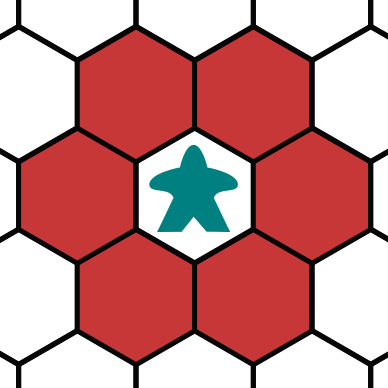
\includegraphics{graphics/tackle-zones-1.png}
    \caption{The reach around a player.}
    \label{fig:tackle-zone-1}
\end{figure}

\begin{figure}
    \centering
    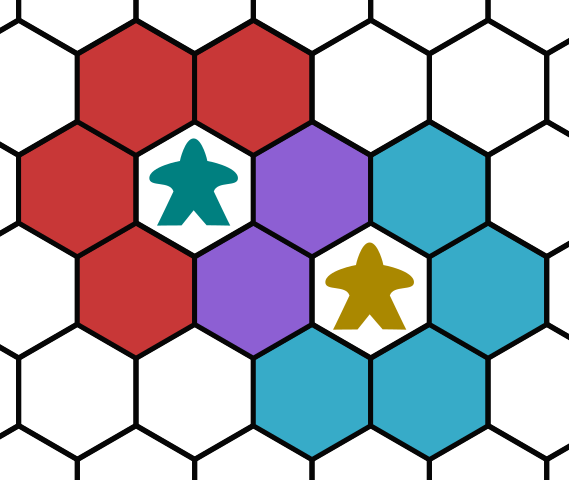
\includegraphics{graphics/tackle-zones-2.png}
    \caption{The overlapping reaches between two players.}
    \label{fig:tackle-zone-2}
\end{figure}